%% Copernicus Publications Manuscript Preparation Template for LaTeX Submissions
%% ---------------------------------
%% This template should be used for copernicus.cls
%% The class file and some style files are bundled in the Copernicus Latex Package which can be downloaded from the different journal webpages.
%% For further assistance please contact the Copernicus Publications at: publications@copernicus.org
%% http://publications.copernicus.org


%% Please use the following documentclass and Journal Abbreviations for Discussion Papers and Final Revised Papers.

%% 2-Column Papers and Discussion Papers
\documentclass[gmd, manuscript]{copernicus}

%% Journal Abbreviations (Please use the same for Discussion Papers and Final Revised Papers)

% Archives Animal Breeding (aab)
% Atmospheric Chemistry and Physics (acp)
% Advances in Geosciences (adgeo)
% Advances in Statistical Climatology, Meteorology and Oceanography (ascmo)
% Annales Geophysicae (angeo)
% ASTRA Proceedings (ap)
% Atmospheric Measurement Techniques (amt)
% Advances in Radio Science (ars)
% Advances in Science and Research (asr)
% Biogeosciences (bg)
% Climate of the Past (cp)
% Drinking Water Engineering and Science (dwes)
% Earth System Dynamics (esd)
% Earth Surface Dynamics (esurf)
% Earth System Science Data (essd)
% Fossil Record (fr)
% Geographica Helvetica (gh)
% Geoscientific Instrumentation, Methods and Data Systems (gi)
% Geoscientific Model Development (gmd)
% Geothermal Energy Science (gtes)
% Hydrology and Earth System Sciences (hess)
% History of Geo- and Space Sciences (hgss)
% Journal of Sensors and Sensor Systems (jsss)
% Mechanical Sciences (ms)
% Natural Hazards and Earth System Sciences (nhess)
% Nonlinear Processes in Geophysics (npg)
% Ocean Science (os)
% Proceedings of the International Association of Hydrological Sciences (piahs)
% Primate Biology (pb)
% Scientific Drilling (sd)
% SOIL (soil)
% Solid Earth (se)
% The Cryosphere (tc)
% Web Ecology (we)
% Wind Energy Science (wes)


%% \usepackage commands included in the copernicus.cls:
%\usepackage[german, english]{babel}
% \usepackage{tabularx}
%\usepackage{cancel}
%\usepackage{multirow}
%\usepackage{supertabular}
%\usepackage{algorithmic}
%\usepackage{algorithm}
%\usepackage{amsthm}
%\usepackage{float}
%\usepackage{subfig}
%\usepackage{rotating}
% \usepackage{graphicx}
\usepackage{hyperref}
% \DeclareGraphicsExtensions{.pdf, .png, .jpg, .eps}
\graphicspath{ {./figs/} }
%
% \usepackage{lineno}
% \linenumbers*[1]
%
% \begin{linenomath*}
% \begin{equation}
% \end{equation}
% \end{linenomath*}

\begin{document}

\title{The Variable Infiltration Capacity (VIC) Model, Version 5.0 - Improvements and New Applications}

% \Author[affil]{given_name}{surname}
\Author[1,2]{Joseph J.}{Hamman}
\Author[1]{Bart}{Nijssen}
\Author[3]{Theodore}{Bohn}
\Author[1]{Diana}{Gergel}
\Author[1]{Yixin}{Mao}

\affil[1]{Department of Civil \& Environmental Engineering, University of Washington, Seattle, WA, USA.}
\affil[2]{Hydrometeorological Applications Program, Research Applications Laboratory, National Center for Atmospheric Research, Boulder, Colorado, USA}
\affil[3]{School of Earth and Space Exploration, Arizona State University, Tempe, AZ, USA.}

%% The [] brackets identify the author with the corresponding affiliation. 1, 2, 3, etc. should be inserted.



\runningtitle{VIC 5.0 - IMPROVEMENTS AND NEW APPLICATIONS}

\runningauthor{HAMMAN ET AL.}

\correspondence{Bart Nijssen (nijssen@uw.edu)}



\received{}
\pubdiscuss{} %% only important for two-stage journals
\revised{}
\accepted{}
\published{}

%% These dates will be inserted by Copernicus Publications during the typesetting process.


\firstpage{1}

\maketitle



\begin{abstract}
  The Variable Infiltration Capacity (VIC) model is a macro-scale semi-distributed hydrologic model.
  VIC development began in the early 1990s and it has since been used extensively, applied from basin to global scales.
  VIC has been applied in a many use cases, including hydrologic data set construction, trend analysis, data evaluation and assimilation, forecasting, coupled climate modeling, and climate change impact analysis.
  Ongoing operational applications of the VIC model include the University of Washington's drought monitor and forecast systems, and NASA's land data assimilation systems.
  This paper outlines the development of VIC version 5, which included a major reconfiguration of the legacy VIC source code to support a wider range of modern modeling applications.
  The VIC source code has been moved to a public Github repository to encourage participation by the broader user and developer.
  The reconfiguration has separated the physical core of the model from the driver, which is responsible for memory allocation, pre- and post-processing and I/O.
  VIC 5 includes four drivers that use the same physical model core: classic, image, CESM, and Python.
  The classic driver supports legacy VIC configurations and runs in the traditional time-before-space configuration.
  The image driver includes a space-before-time configuration, NetCDF I/O, and uses MPI for parallel processing.
  This configuration will facilitate the direct coupling of streamflow routing, reservoir operation, and irrigation processes within VIC.
  The image driver is the foundation of the CESM driver; which couples VIC to the Community Earth System Model's (CESM) flux coupler (CPL7) and a prognostic atmosphere.
  The Python driver provides interactive access to the functions and datatypes of VIC's physical core from a Python interface.
  Finally, VIC 5.0 is distributed with a robust test infrastructure, components of which routinely run during development using the Travis CI continuous integration service.
  The work described here represents a major step forward for the VIC user community in terms of support for both existing and new model applications.
\end{abstract}

\introduction
  The Variable Infiltration Capacity (VIC) model \citep{Liang_1994} is a macro-scale semi-distributed hydrologic model.
  This paper introduces VIC version 5, a new major release of the VIC model.
  The goals of this paper are to describe the software, infrastructure, and science improvements to the version 5 release of the VIC model and to provide baseline model diagnostics.
  The initial VIC 5 release does not add new physical representation compared to the last release of VIC 4 development track (version 4.2.d).
  Instead, the development of VIC version 5 focused on reconfiguring the legacy VIC source code to support a wider range of modern modeling applications.

  VIC has been applied in a broad set of use cases.
  Examples of VIC applications include the construction of hydrologic data sets, trend analysis, data evaluation and assimilation, forecasting, coupled climate modeling, and climate change impact analysis.
  The VIC model has been tested extensively using point observational data from sites like the First ISLSCP Field Experiment \citep[FIFE;][]{Liang_1994}, and through participation in the World Climate Research Program (WCRP) Project for the Intercomparison of Land Parameterization Schemes \citep[PILPS;][]{Bowling_2003,wood_1998}.
  The model has been used for numerous water and energy balance studies in the U.S. \citep{Abdulla_1997,Nijssen_1997}, the arctic \citep{Adam_2008,Su_2005,Tan_2011,Hamman_2016a} and globally \citep{Nijssen_2001a,Nijssen_2001b,Nijssen_2001c,Sheffield_2009}.
  One result of these studies has been refinement of the model to better represent key hydrological processes \citep{Andreadis_2009,Cherkauer_2003,Liang_1996,Liang_1999}.
  Ongoing realtime applications of the VIC model include the University of Washington’s Drought Monitor and forecast systems (\url{http://hydro.washington.edu/forecast/monitor/drought/index.shtml}), and NASA’s land data assimilation systems (\url{http://ldas.gsfc.nasa.gov/nldas/}).
  Table \ref{table:vic_applications} provides additional examples of the use of VIC for hydrological, water resources, and water and energy budget applications.

  Although the original VIC publication \citep{Liang_1994} indicated its applicability within coupled land-atmosphere models, VIC has predominantly been applied in uncoupled modeling studies.
  As a result, the software infrastructure surrounding the released version of the model has not been updated to support modern scientific computing tools such as parallel processing or advanced data formats (e.g NetCDF).
  The main loop order in the model was originally written in a time-before-space orientation.
  This configuration simplified the memory management within the model and facilitated parallelization without the use of multiprocessing software.
  For these reasons, VIC applications within multi-model frameworks \citep[e.g. NASA LIS, ][]{Kumar_2006} and coupled land-atmosphere models \citep[e.g. RASM, ][]{Hamman_2016a} have therefore required significant custom reconfiguration of the model interface.

  \subsection{The VIC Community and Open Source}
    \label{sec:vic_community}
    The VIC Users email list-serve (\url{vic_users@u.washington.edu}) has more than 375 active members.
    Analytics from the VIC website and documentation indicates that there are upwards of one-thousand individual VIC users (Figure \ref{fig:vic_users}a).
    Citations of the original \citep{Liang_1994} continue to increase (Figure \ref{fig:vic_users}b).
    Since the VIC source code has been available in a public GitHub repository, over 100 users have checked out ``Forks''.
    Additionally, we are aware of a multiple ongoing developing efforts by the VIC community to implement new features.
    The open source framework that we have implemented will facilitate mechanisms for the integration of model improvements from the greater VIC community into future VIC releases.

    Beginning in 2011, the VIC model has been licensed with the open source GNU General Public License version 2.
    The motivation behind making the model source code completely open-source was to encourage participation by the model user and development community-at-large, and to increase scientific transparency in the model development and application process \citep{Ince_2012}.
    The VIC source code now uses the Git version control system \citep{Torvalds_2010} and is publicly available on Github (\url{https://github.com/UW-Hydro/VIC}).
    While the majority of the VIC 5 development was done by researchers at the University of Washington, a number features and bug fixes were made by unsolicited contributors.

\section{Data and Model Simulations}
  \label{sec:data_and_sims}
  In this paper, we demonstrate the VIC model performance using three existing VIC model configurations: N.America, RASM, and Global.
  These model configurations are shown in Figure \ref{fig:vic_domains} and are detailed in Table \ref{table:model_sims}.
  Scientific validation of the VIC 5 release includes point comparisons of VIC simulations with 66 FluxNET observations and 448 SNOTEL observations.
  % These comparison datasets are available...actually, we need to figure out if we can distribute these datasets.

\section{Model Improvements}
  \label{sec:improvements}
  The VIC 5 release includes a complete refactor of the model source code.
  The reconfiguration has separated the physical core of the model from the driver, which is responsible for memory allocation, pre- and post-processing, and input and output (I/O).
  The VIC 5 source code structure is depicted in Figure \ref{fig:vic_config}.
  The initial VIC 5 release includes four drivers, each using the same physical model core:
  \begin{enumerate}
    \item \textit{Classic Driver}: The \textit{Classic Driver} supports legacy VIC configurations and runs in the traditional time-before-space configuration.
    It uses the ASCII and flat-binary file formats for I/O.
    \item \textit{Image Driver}: The \textit{Image Driver} includes a space-before-time configuration, NetCDF I/O \citep{Rew_1990}, and uses MPI for parallel processing \citep{Gropp_1996}.
    This configuration facilitates the direct coupling of streamflow routing, reservoir, and irrigation processes within VIC.
    \item \textit{CESM Driver}: The \textit{Image Driver} is the foundation of the CESM driver; which couples VIC to Community Earth System Model's \citep[CESM;][]{Hurrell_2013} flux coupler \citep[CPL7;][]{Craig_2012} and a prognostic atmosphere.
    The initial application of the \textit{CESM Driver} is within the Regional Arctic System Model (RASM) \citep{Hamman_2016a}, a regional implementation of CESM.
    Future applications of the \textit{CESM Driver} could easily be applied within the global version of CESM.
    \item \textit{Python Driver}: Finally, we have added a Python bindings that provide access to the functions and datatypes of VIC’s physical core from a Python interface.
    Although the \textit{Python Driver} is currently only used for testing, this driver is uniquely suited for future data assimilation and large ensemble applications.
  \end{enumerate}

  We have also introduced a model extensions framework to facilitate the coupling of sub-model components, such as streamflow routing, reservoirs, irrigation, glaciers and ice sheets, and dynamic vegetation and crops.
  The motivating factor for developing this framework was to allow for the option coupling of existing sub-models that are beyond the scope of core VIC applications or that are not feasible to add for all drivers.
  These extensions are generally compile time options.

  \subsection{Parallel Computing}
    \label{sec:mpi}
    The VIC model does not include horizontal transport between grid cells.
    In the past, this feature has allowed users to manually parallelize their VIC applications by running VIC simulations on completely separate computers, if need be.
    Included in the image and CESM drivers in VIC 5, we have added formal parallel processing support utilizing the Message Passing Interface (MPI) standard \citep{Gropp_1996}.
    Leveraging the independence of VIC grid points in terms of neighbor communication (i.e. horizontal transport between grid cells), the parallelization strategy that we have adopted only uses MPI utilities to facilitate I/O operations.
    Shared memory between MPI tasks is limited to model settings.

    Figure \ref{fig:vic_scaling} demonstrates the scaling performance of the parallelization scheme applied in VIC 5 in terms model runtime and memory usage for the N.America, RASM, and Global model configurations.
    Memory usage is modest in VIC since it is basically a 2d model [add maximum memory usage for each test domain].
    Parallelization is therefor mostly for I/O, facilitating single processor reads and writes.
    Consequently, the scaling is mostly a function of the computer's interconnect and disk speed.
    [Throughput and strong scaling (defined as a percentage of perfectly linear scaling, e.g.  t1 / ( N * tN ) * 100\%)]
    [Complete once all scaling tests have been written.]

    We expect the scaling performance of the VIC image and CESM drivers to be further improved by the application of parallel IO and shared-memory parallel programming such as OpenMP.
    Collective parallel reading and writing of netCDF files, made possible through the NetCDF-4 and HDF5 libraries, will dramatically reduce the amount of data passed via MPI processes and, in theory, should allow the model to scale well beyond the limits shown in Figure \ref{fig:vic_scaling}.
    The initial parallelization of VIC has not applied any on-node shared-memory threading.
    Because there is a certain amount of overhead associated with each MPI library call, we also expect that the application of a threading library, such as OpenMP, will lead to additional improvements in the model performance.

  \subsection{Input and Output}
    \label{sec:io}
    The Image and CESM drivers use the NetCDF library for all I/O related to input parameters, meteorological forcings, and model output.
    NetCDF is a software library that reads and writes array-oriented scientific data.
    It has been widely adopted among the geo-scientific modeling community and provides a convenient self-describing machine-independent data format.
    Output files from the Image and CESM drivers are formatted such that they meet the NetCDF Climate and Forecast (CF) metadata conventions version 1.6 \citep{Eaton_2003}.
    The classic driver continues to support the legacy ASCII and binary input and output file formats.
    We have also added additional metadata to the ASCII file formats but they have basically remained the same since VIC 4.

    VIC 5 also has eliminated all hard coded model parameters from the body of the source code.
    Users may now specify an optional ``parameters'' configuration file to set non-default model constants that were previously hard-coded values.
    This feature greatly improves the transparency and accessibility of the model.

  \subsection{Testing}
    \label{sec:testing}
    VIC 5 introduces a robust test suite, now distributed with the model source code.
    The test suite is made up of six components:

    \begin{enumerate}
      \item \textit{Unit}: Unit tests are tests that check function level source code behavior.
      Using the Python Driver, many of the individual functions in VIC are tested for using the ``Py-Test'' unit test framework (\url{http://doc.pytest.org/}).
      \item \textit{System}: The system tests check the behavior of the individual drivers.
      Examples of these tests include checks for exact restarts, binary equivalence for simulations run with and without MPI, and comparisons between drivers.
      \item \textit{Science}: The science tests utilize the classic driver to run point simulations at a selection of observation locations (e.g. SNOTEL or AMERIFLUX).
      Results from these point simulations are quantitatively and qualitatively compared to observations and previous VIC model results (e.g. Figure \ref{fig:vic_4v5}).
      \item \textit{Examples}: A set of short example VIC configurations and inputs are provided to users for the Classic and Image drivers.
      The Examples tests simply check that the example data continue to run so that users can easily get started with the VIC model.
      \item \textit{Release}: The release tests are longer, full domain (e.g. N.America, Global, etc.) simulations performed prior to release.
      These tests demonstrate the current model behavior and are compared to previous releases to demonstrate the changes in the model physics.
      \item \textit{Performance}: With the addition of MPI to the Image and CESM drivers, a set of tools for assessing the parallel performance were needed.
      The performance tests asses timing and memory statistics of the VIC model.
      Results from these tests are highlighted in Section \ref{sec:mpi}.
    \end{enumerate}

    A subset of these tests are routinely run using the Travis CI continuous integration system ( \url{https://travis-ci.org/}).
    As the VIC developer community grows, this test suite will be an important tool in maintaining the function of the supported drivers.

\section{New Applications}
  \label{sec:new_apps}
  The development of VIC 5 has enabled a series of new or improved model applications.
  These applications include the coupling of VIC to atmospheric models, incorporation within multi-model frameworks, or application of model sub-components that have previously been difficult to apply.
  Here we highlight a few of these new applications that we think are likely to be implemented:

  \subsection{Multi-model Frameworks}
    \label{sec:multimodel}
    Multi-model frameworks such as NASA's LIS \citep{Kumar_2006}, WRF-Hydro \citep{Gochis_2013}, or the Community Surface Dynamics Modeling System \citep{Peckham_2016} have allowed the modeling community the opportunity to run simulations with multiple models from a consistent interface.
    While previous versions of VIC have been included in LIS, the model version is seldom updated due to the tedious nature of the work.
    The reconfiguration of VIC 5 greatly simplifies the application of VIC within these frameworks and we expect that both will incorporate the new model version.

  \subsection{Coupled Land-Atmosphere Modeling}
    \label{sec:coupled_apps}
    One of the primary motivating factors in the development of VIC 5 was to enable coupling of VIC within RASM and CESM.
    In RASM, VIC 5 is directly coupled to CESM's flux coupler (CPL7).
    This coupling allows VIC to be run with WRF as the atmospheric component.
    VIC may also be coupled to NASA's Nu-WRF through the LIS framework described above.
    At the time of writing, the coupling of VIC with Nu-WRF has not begun.

  % Perhaps add a section on Forecast and Data-assimilation Applications
  % \subsection{Forecast and Data-assimilation Applications}
  %   \label{sec:forecast_apps}

\conclusions[Discussion and Conclusions]
  Figure \ref{fig:vic_4v5} demonstrates that VIC 4 and VIC 5 are producing similar results.
  The two model versions have similar performance statistics when compared to observations.
  \textit{Diana, let's get together to think of a few summary figures that 1) demonstrate that VIC 4 and 5 are behaving the same, and 2) summarize the science test simulations in an interesting way.}

  Figure \ref{fig:vic_domain_results} demonstrates that VIC 5 is producing plausible results on a variety of spatial domains.
  \textit{Yixin, let's get together to think of a way to demonstrate that VIC 5 has been run for each of the configurations for this paper and that the results.}

  The updated model configuration facilitates the direct coupling new and existing subcomponents to VIC.
  Work currently underway is using the extensions framework discussed in Section \ref{sec:improvements} to tightly couple the RVIC streamflow routing model with the image driver.
  Future extension development is also expected to add reservoirs, irrigation, glaciers, dynamic vegetation, and crop models to VIC.
  While some of these had been partially developed with VIC 4, the limitations imposed by the lack of infrastructure have preclude their wider application in the VIC community.

  With the open-source status of VIC and the release of VIC 5, we hope to see growing community presence in the maintenance and development of the model.

\section{Code Availability}
\label{appendix:code_avail}

  Appendix \ref{appendix:source_code} describes the locations and license information for the the VIC source code and documentation.
  The source code, input data, and VIC configurations used as demonstrations for this paper, are provided in this Github repository: \url{https://github.com/jhamman/VIC5_paper}.

\appendix
\section{VIC Model Source Code and Documentation}
\label{appendix:source_code}
{\bf Archive}

\begin{itemize}
	\item \textit{Name}: VIC.5.0.0
	\item \textit{Persistent identifier}: 10.5281/zenodo.61423
	\item \textit{License}: GNU General Public License, version 2 (GPL-2.0)
	\item \textit{Publisher}:  Zenodo
	\item \textit{Version published}: 5.0.0
	\item \textit{Date published}: September 2, 2016
\end{itemize}

{\bf Code Repository}

\begin{itemize}
	\item \textit{Name}: GitHub
	\item \textit{Identifier}: \url{https://github.com/UW-Hydro/VIC/}
	\item \textit{License}: GNU General Public License, version 2 (GPL-2.0)
	\item \textit{Date published}: September 2, 2016
\end{itemize}

{\bf Versioned Documentation}

\begin{itemize}
	\item \textit{Name}: ReadTheDocs
	\item \textit{Identifier}: \url{http://vic.readthedocs.io/en/vic.5.0.0/}
	\item \textit{License}: GNU General Public License, version 2 (GPL-2.0)
	\item \textit{Date published}: September 2, 2016
\end{itemize}

% \subsection{}                               %% Appendix A1, A2, etc.

\authorcontribution{J. Hamman, B. Nijssen, and T. Bohn performed the majority the source code reconfiguration. J. Hamman, J. Hamman designed the experiments with help from Y. Mao and D. Gergle to carry them out. J. Hamman prepared the manuscript with contributions from all co-authors.}

\begin{acknowledgements}
  This research was supported, in part, under United States Department of Energy (DOE) grants DE-FG02-07ER64460 and DE-SC0006856 to the University of Washington, and grant 1216037 of the National Science Foundation's Science, Engineering, and Education for Sustainability (SEES) Program.
\end{acknowledgements}


%% REFERENCES

%% The reference list is compiled as follows:

% \begin{thebibliography}{}
%
% \bibitem[AUTHOR(YEAR)]{LABEL}
% REFERENCE 1
%
% \bibitem[AUTHOR(YEAR)]{LABEL}
% REFERENCE 2
%
% \end{thebibliography}

%% Since the Copernicus LaTeX package includes the BibTeX style file copernicus.bst,
%% authors experienced with BibTeX only have to include the following two lines:
%%
\bibliographystyle{copernicus}
\bibliography{biblio}
%%
%% URLs and DOIs can be entered in your BibTeX file as:
%%
%% URL = {http://www.xyz.org/~jones/idx_g.htm}
%% DOI = {10.5194/xyz}


%% LITERATURE CITATIONS
%%
%% command                        & example result
%% \citet{jones90}|               & Jones et al. (1990)
%% \citep{jones90}|               & (Jones et al., 1990)
%% \citep{jones90,jones93}|       & (Jones et al., 1990, 1993)
%% \citep[p.~32]{jones90}|        & (Jones et al., 1990, p.~32)
%% \citep[e.g.,][]{jones90}|      & (e.g., Jones et al., 1990)
%% \citep[e.g.,][p.~32]{jones90}| & (e.g., Jones et al., 1990, p.~32)
%% \citeauthor{jones90}|          & Jones et al.
%% \citeyear{jones90}|            & 1990



%% FIGURES

%% ONE-COLUMN FIGURES

%%f
\begin{figure}[t]
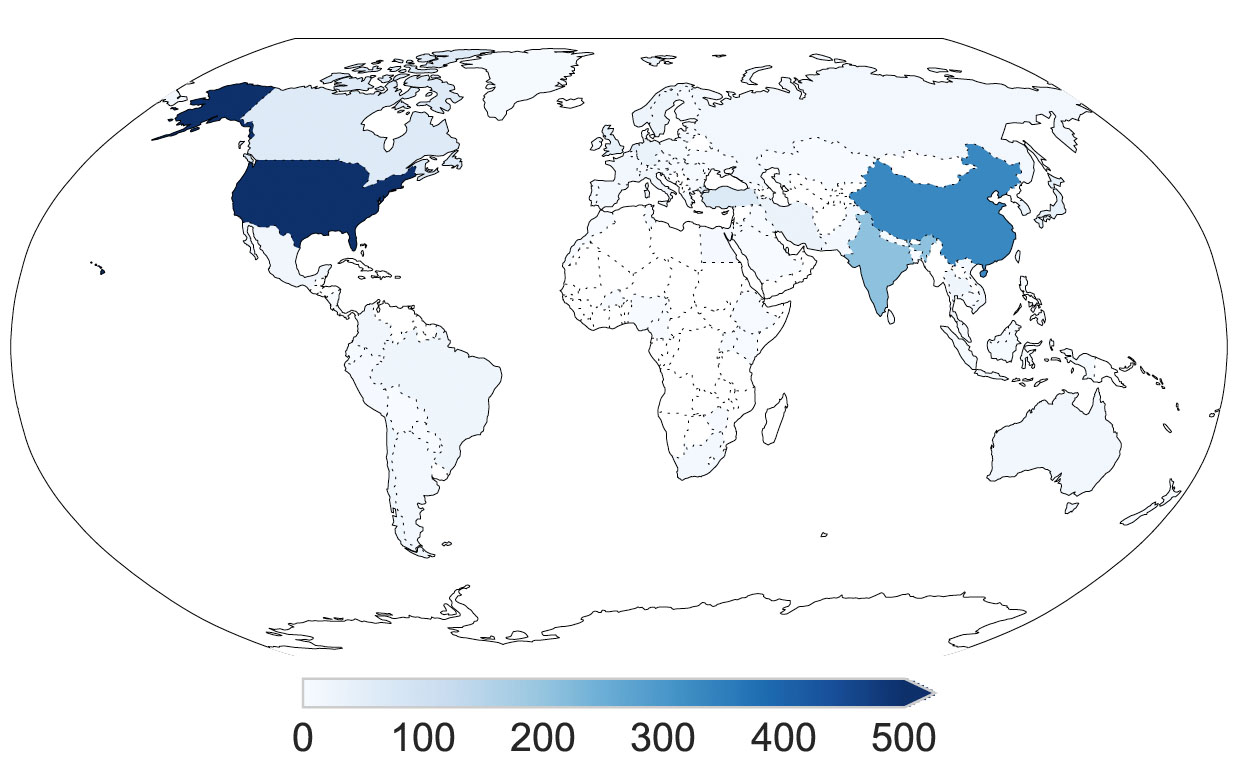
\includegraphics[width=8.3cm]{VIC_users.jpg}
\caption{Number of unique visitors to the VIC documentation website (\url{http://vic.readthedocs.org}) between September 1, 2015 and November 31, 2015. Data from Google Analytics (\url{https://analytics.google.com}).}
\label{fig:vic_users}
\end{figure}

\begin{figure}[t]
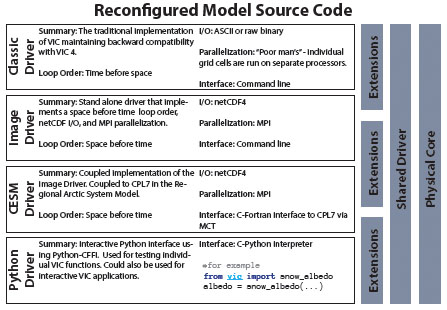
\includegraphics[width=8.3cm]{VIC_config.jpg}
\caption{VIC source code structure after reconfiguration. }
\label{fig:vic_config}
\end{figure}

%
%%% TWO-COLUMN FIGURES
%
%f
\begin{figure}[t]
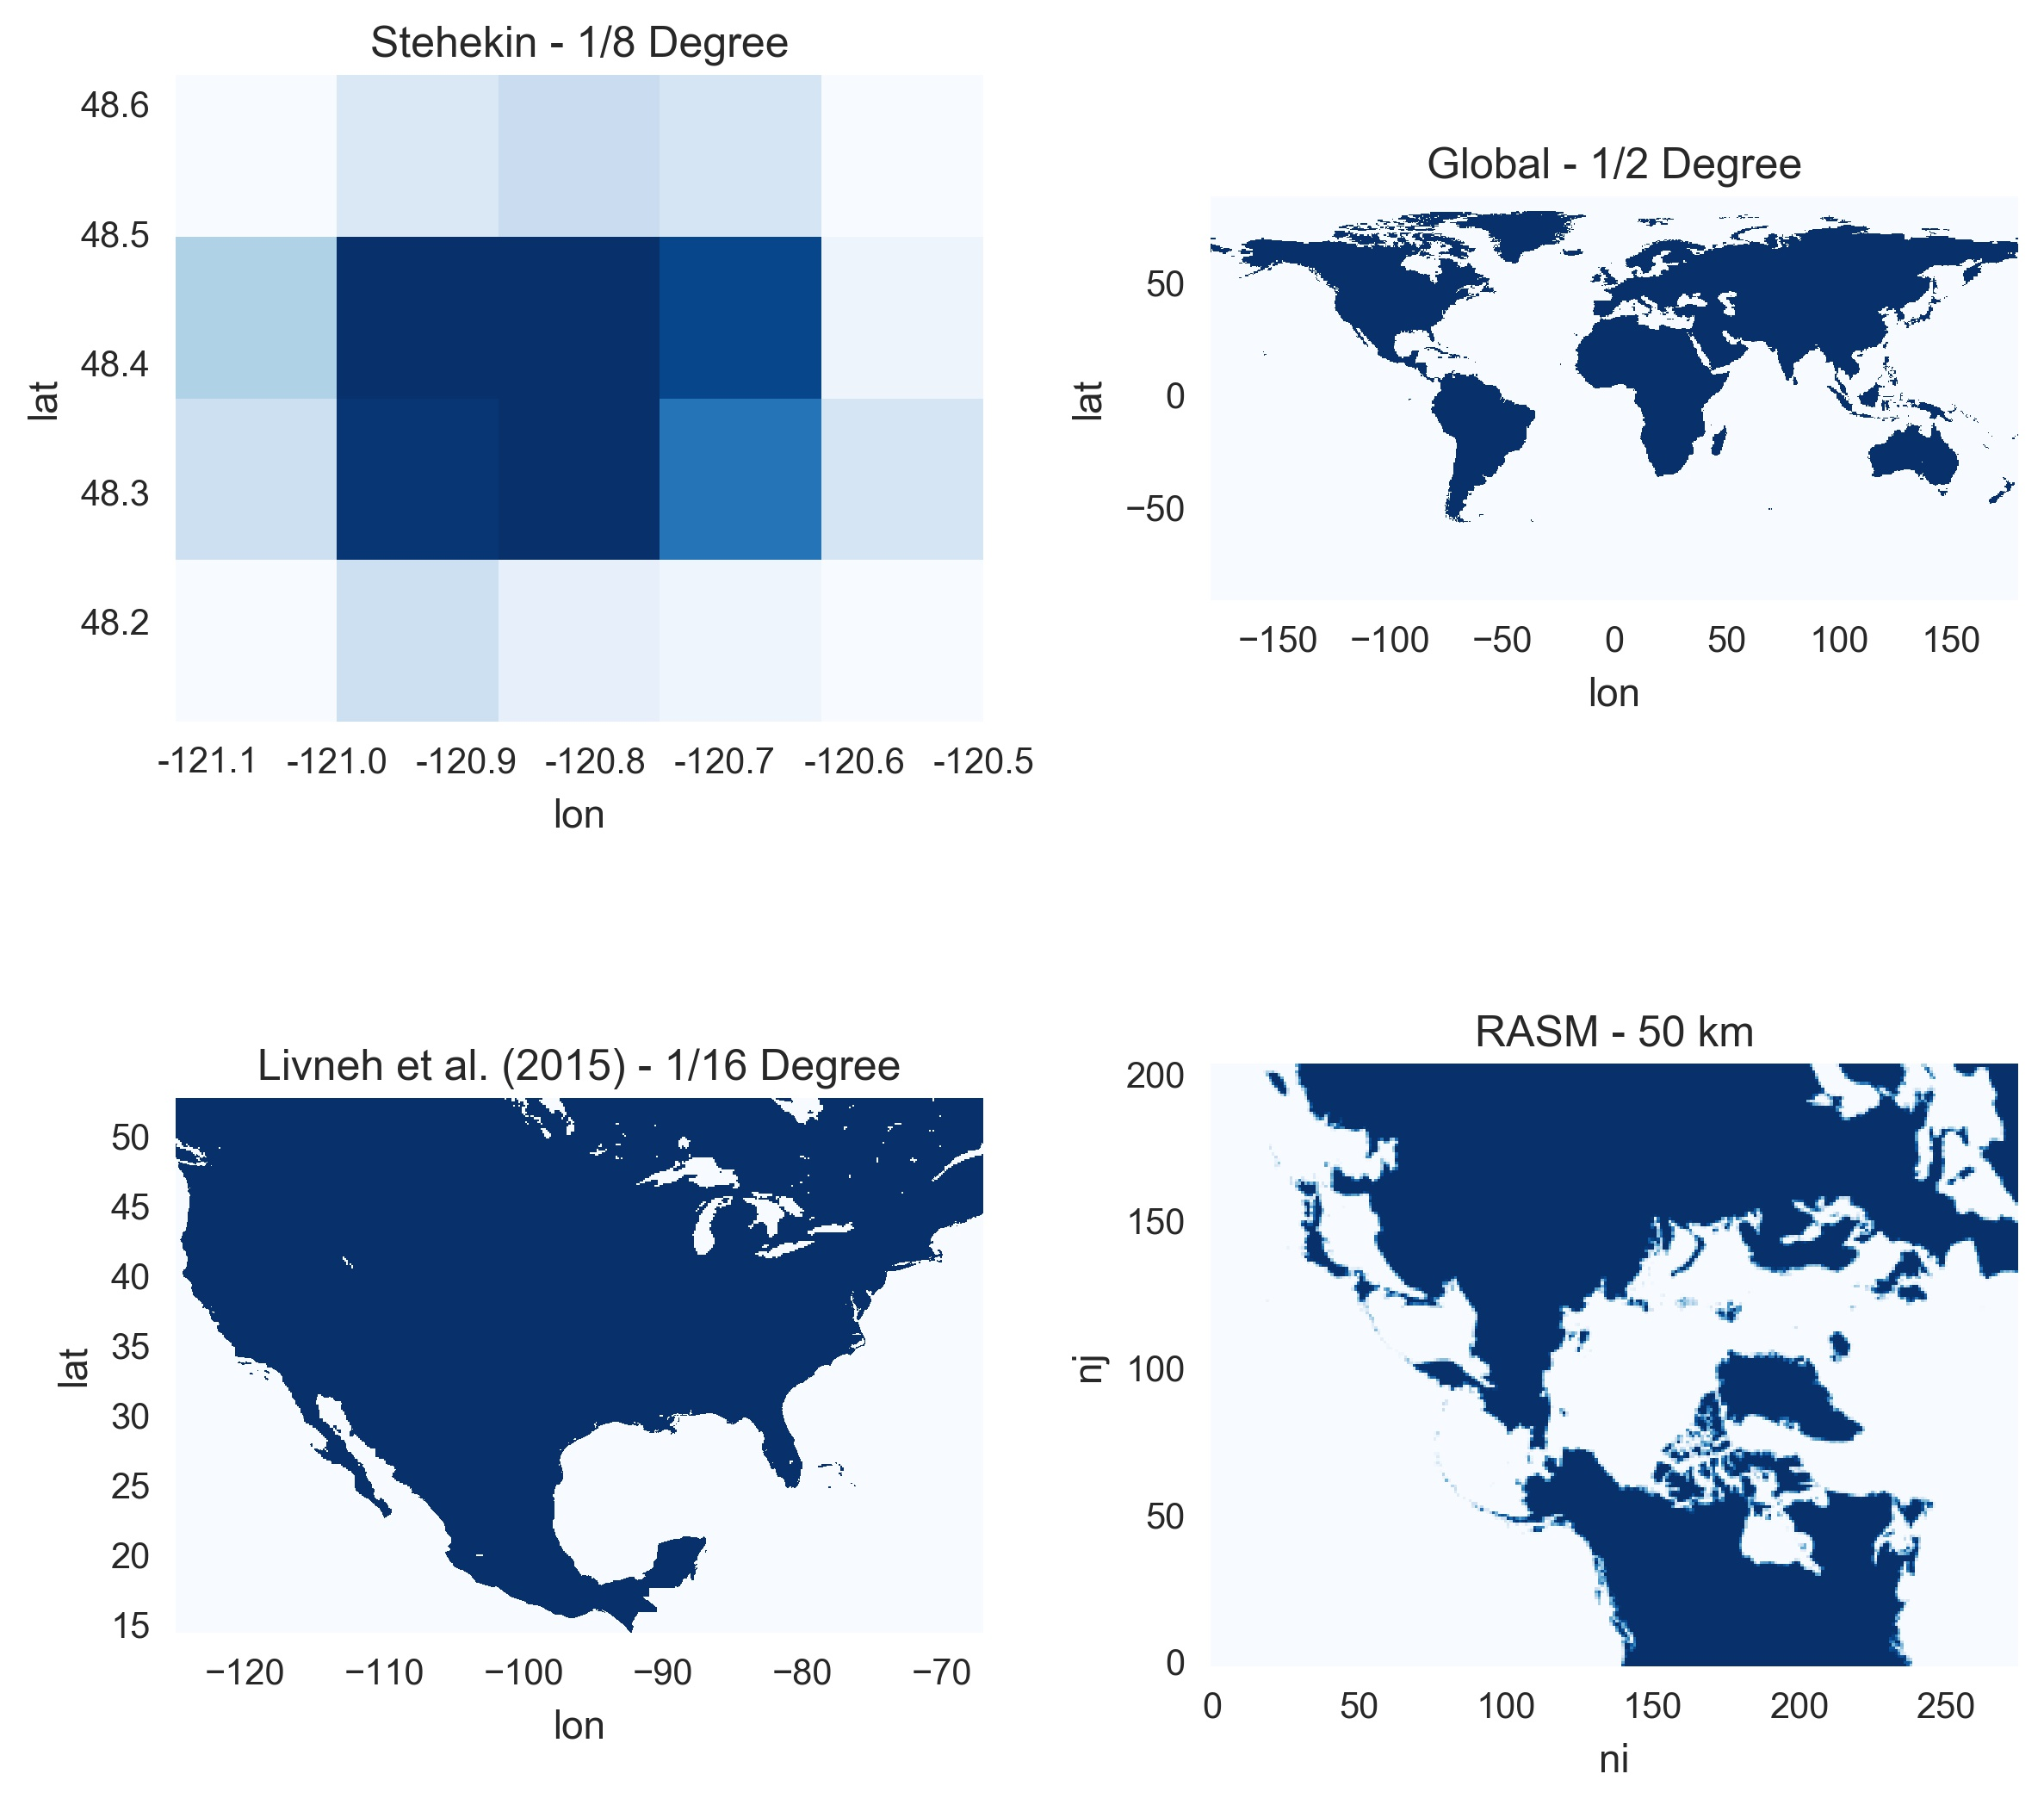
\includegraphics[width=8.3cm]{VIC_domains.jpg}
\caption{TEXT}
\label{fig:vic_domains}
\end{figure}

\begin{figure}[t]
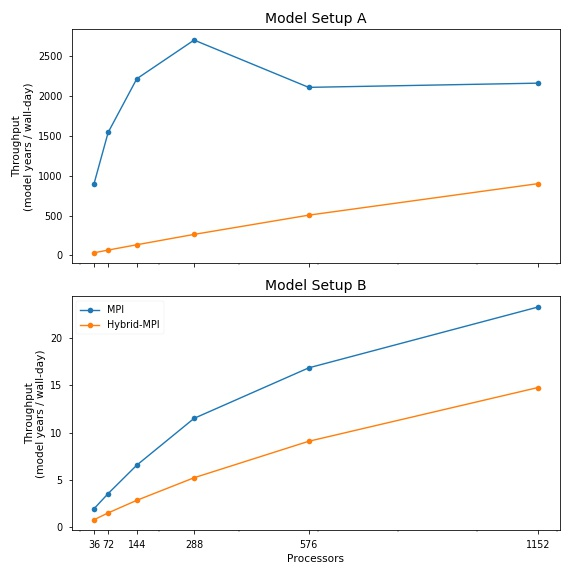
\includegraphics[width=8.3cm]{VIC_scaling.jpg}
\caption{TEXT}
\label{fig:vic_scaling}
\end{figure}

\begin{figure*}[t]
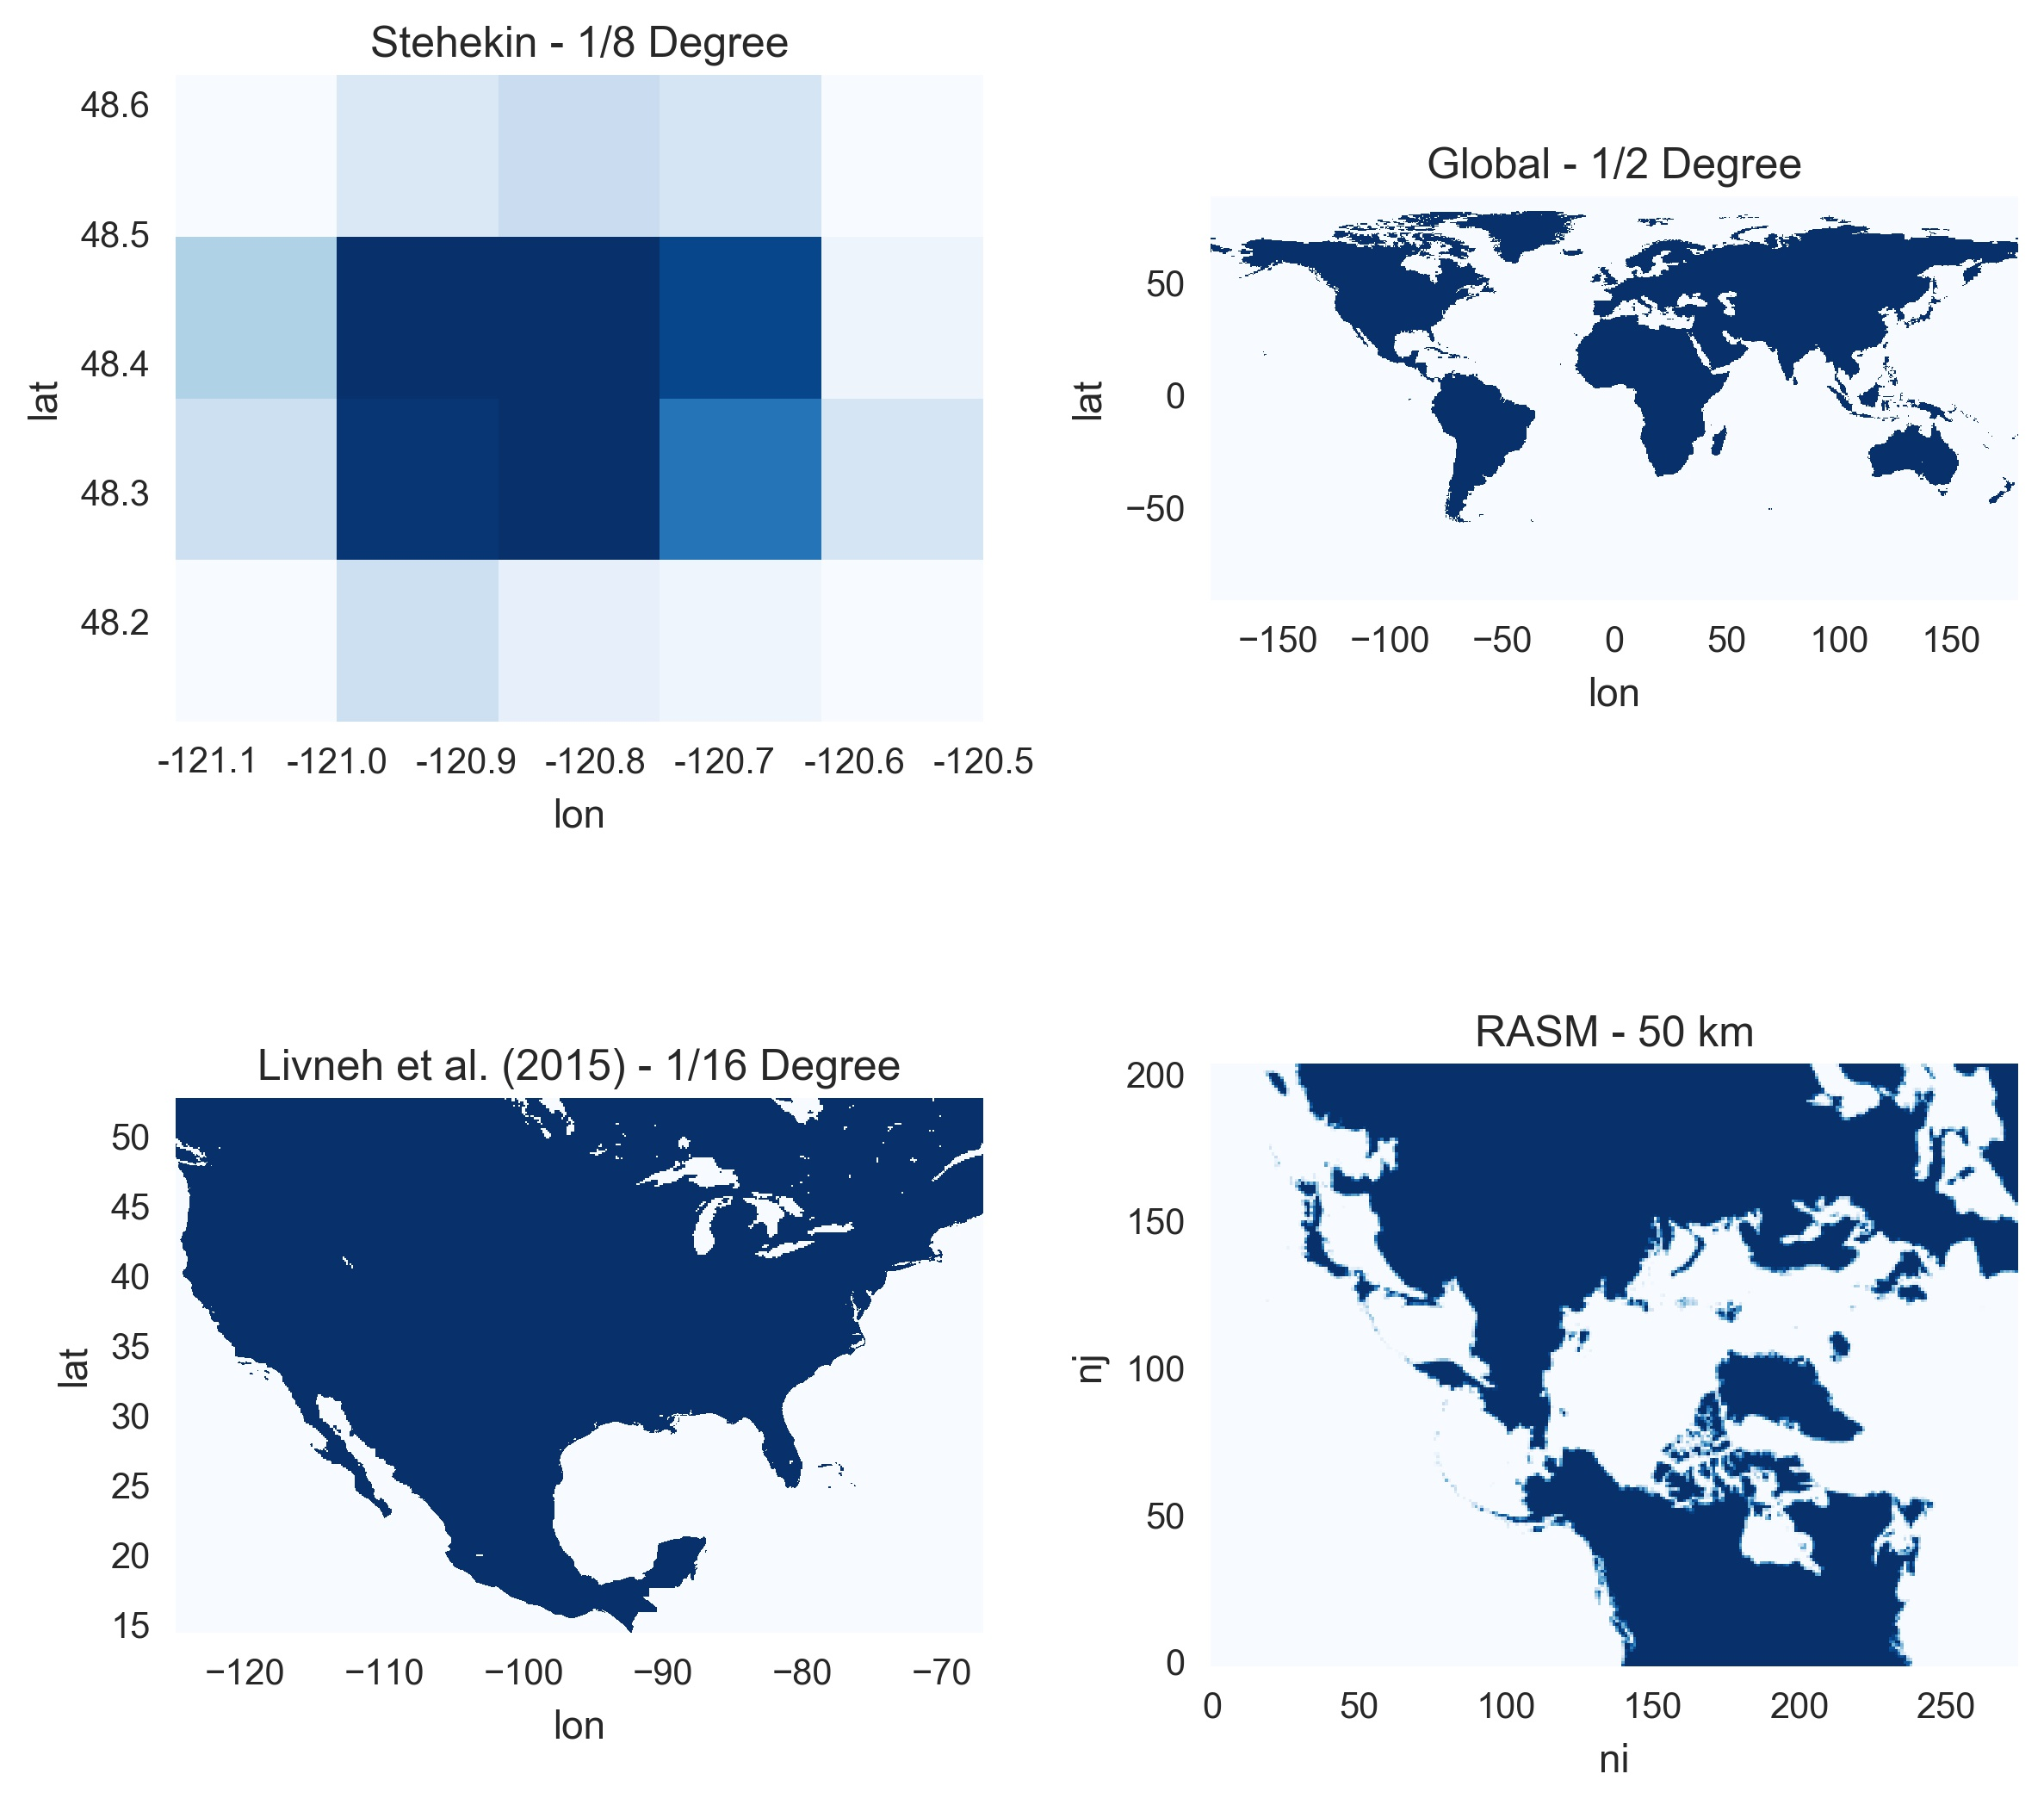
\includegraphics[width=12cm]{VIC_domains.jpg}
\caption{TEXT}
\label{fig:vic_domain_results}
\end{figure*}

\begin{figure*}[t]
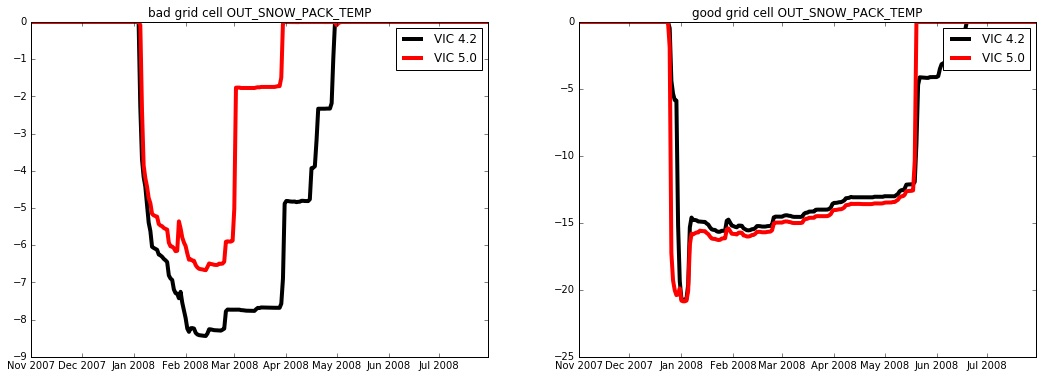
\includegraphics[width=12cm]{VIC_4v5.jpg}
\caption{TEXT}
\label{fig:vic_4v5}
\end{figure*}

%
%
%%% TABLES
%%%
%%% The different columns must be seperated with a & command and should
%%% end with \\ to identify the column brake.
%
%%% ONE-COLUMN TABLE
%
\clearpage
\begin{table}[]
  \caption{Examples of VIC applications}
  \label{table:vic_applications}
  \resizebox{\textwidth}{!}{%
  \begin{tabular}{ll}
    \hline
    \multicolumn{2}{l}{\textbf{Data set construction}}                                                                                                              \\ \hline
    \multicolumn{1}{l|}{US}                      & \citet{Maurer_2002}  \\ \hline
    \multicolumn{1}{l|}{Global}                  & \citet{Nijssen_2001a,Nijssen_2001c,Sheffield_2006}  \\ \hline
    \multicolumn{1}{l|}{Arctic}                  & \citet{Hamman_2016b} \\ \hline
    \multicolumn{2}{l}{\textbf{Historic trend analysis}}                                                                                                            \\ \hline
    \multicolumn{1}{l|}{Snow}                    & \citet{Hamlet_2005,Shi_2011}  \\ \hline
    \multicolumn{1}{l|}{Land use/cover change}   & \citet{Matheussen_2000}  \\ \hline
    \multicolumn{1}{l|}{Streamflow}              & \citet{Hamlet_2007a,Hamlet_2007b,Tan_2011}  \\ \hline
    \multicolumn{1}{l|}{Drought}                 & \citet{Gao_2011,Sheffield_2007,Sheffield_2008,Sheffield_2009,Wang_2011,Nijssen_2014}  \\ \hline
    \multicolumn{2}{l}{\textbf{Data evaluation}}                                                                                                                    \\ \hline
    \multicolumn{1}{l|}{Satellite precipitation} & \citet{Nijssen_2004,Pan_2010,Su_2008}  \\ \hline
    \multicolumn{1}{l|}{Reanalysis}              & \citet{Maurer_2001}  \\ \hline
    \multicolumn{2}{l}{\textbf{Data assimilation}}                                                                                                                  \\ \hline
    \multicolumn{1}{l|}{Snow}                    & \citet{Andreadis_2006}  \\ \hline
    \multicolumn{1}{l|}{Soil moisture}           & \citet{Pan_2006}  \\ \hline
    \multicolumn{2}{l}{\textbf{Forecasting and nowcasting}}                                                                                                         \\ \hline
    \multicolumn{1}{l|}{Droughts}                & \citet{Shukla_2011}  \\ \hline
    \multicolumn{1}{l|}{Streamflow}              & \citet{Hamlet_1999,Li_2009,Wood_2002}  \\ \hline
    \multicolumn{1}{l|}{Predictability}          & \citet{Gebregiorgis_2011,Maurer_2003}  \\ \hline
    \multicolumn{2}{l}{\textbf{Climate change impact analysis}}                                                                                                     \\ \hline
    \multicolumn{1}{l|}{Hydrology}               & \citet{Barnett_2005,Beyene_2010,Nijssen_2001b}  \\ \hline
    \multicolumn{1}{l|}{Water resources}         & \citet{Christensen_2007,Christensen_2004,Das_2011,Hamlet_1999}  \\ \hline
    \multicolumn{2}{l}{\textbf{Coupled land-atmosphere modeling}}                                                                                                     \\ \hline
    \multicolumn{1}{l|}{US}                      & \citet{Zhu_2009}                                           \\ \hline
    \multicolumn{1}{l|}{Arctic}                  & \citet{Hamman_2016a} \\ \hline
  \end{tabular}
  }
\end{table}

\clearpage
\begin{table}
  \caption{VIC Model Simulations}
  \centering
  \begin{tabular}{l l l l l}
    \hline
    Model Domain  & Resolution  & Timestep  & Grid Cells  & Forcings  \\
    \hline
    $N.America$     & 1/16th-deg.  & 3-hr.   & 333,579 & Livneh et al. 2015   \\
    $Global$    & 1/2th-deg    & 6-hr.   & 61,345  & CRU-NCEP   \\
    $RASM$      & 50-km        & 20-min. & 25,996  & Sheffield et al. 2006  \\
    $SNOTEL$    & point        & 1-hr    & 448     & In-situ Observations  \\
    $FLUXNET$   & point        & 1-hr    & 66      & In-situ Observations  \\
    \hline
    \label{table:model_sims}
  \end{tabular}
\end{table}

\clearpage
\begin{table}[]
\centering
\caption{Hardware used in VIC Image driver MPI performance tests.}
\label{table:hardware}
\begin{tabular}{|l|c|c|c|}
\hline
                                         & \textbf{Hyak}                                & \textbf{Thunder}                           & \textbf{Gordon}        \\ \hline
\textbf{Operated By}                     & UW                                           & AFRL                                       & Navy DSRC              \\ \hline
\textbf{System}                          & ?                                            & SGI ICE X                                  & Cray XC40              \\ \hline
\textbf{Peak PFlops}                     & ?                                            & 5.62                                       & 2                      \\ \hline
\textbf{Parallel disk storage (Pbytes)}  & ?                                            & 12.2                                       & 2.29                   \\ \hline
\textbf{Total Nodes}                     & $\sim$835                                    & 3,216                                      & 1569                   \\ \hline
\textbf{Operating System}                & RedHat Unix                                  & SGI's Performance Suite                    & Cray Linux Environment \\ \hline
\textbf{Cores/Node}                      & 16                                           & 36                                         & 32                     \\ \hline
\textbf{Core Type}                       & Intel Xeon & Intel Xeon & Intel Xeon \\ \hline
\textbf{Core Speed (GHz)}                & 2.0 - 2.8                                    & 2.3                                        & 2.3                    \\ \hline
\textbf{Memory/Node (Gbytes)}            & 64 - 512                                     & 128                                        & 128                    \\ \hline
\textbf{Accessible Memory/Node (Gbytes)} & 64 - 512                                     & 126                                        & 125                    \\ \hline
\textbf{Memory Model}                    & \multicolumn{3}{c|}{Shared on node. Distributed across cluster.}                                                   \\ \hline
\textbf{Interconnect Type}               & InfiniBand                                   & FDR 14x InfiniBand / Enhanced LX Hypercube & Cray Aries  Dragonfly \\ \hline
\end{tabular}
\end{table}

%
%%% NUMBERING OF FIGURES AND TABLES
%%%
%%% If figures and tables must be numbered 1a, 1b, etc. the following command
%%% should be inserted before the begin{} command.
%
%\addtocounter{figure}{-1}\renewcommand{\thefigure}{\arabic{figure}a}
%
%
%%% MATHEMATICAL EXPRESSIONS
%
%%% All papers typeset by Copernicus Publications follow the math typesetting regulations
%%% given by the IUPAC Green Book (IUPAC: Quantities, Units and Symbols in Physical Chemistry,
%%% 2nd Edn., Blackwell Science, available at: http://old.iupac.org/publications/books/gbook/green_book_2ed.pdf, 1993).
%%%
%%% Physical quantities/variables are typeset in italic font (t for time, T for Temperature)
%%% Indices which are not defined are typeset in italic font (x, y, z, a, b, c)
%%% Items/objects which are defined are typeset in roman font (Car A, Car B)
%%% Descriptions/specifications which are defined by itself are typeset in roman font (abs, rel, ref, tot, net, ice)
%%% Abbreviations from 2 letters are typeset in roman font (RH, LAI)
%%% Vectors are identified in bold italic font using \vec{x}
%%% Matrices are identified in bold roman font
%%% Multiplication signs are typeset using the LaTeX commands \times (for vector products, grids, and exponential notations) or \cdot
%%% The character * should not be applied as mutliplication sign
%
%
%%% EQUATIONS
%
%%% Single-row equation
%
%\begin{equation}
%
%\end{equation}
%
%%% Multiline equation
%
%\begin{align}
%& 3 + 5 = 8\\
%& 3 + 5 = 8\\
%& 3 + 5 = 8
%\end{align}
%
%
%%% MATRICES
%
%\begin{matrix}
%x & y & z\\
%x & y & z\\
%x & y & z\\
%\end{matrix}
%
%
%%% ALGORITHM
%
%\begin{algorithm}
%\caption{�}
%\label{a1}
%\begin{algorithmic}
%�
%\end{algorithmic}
%\end{algorithm}
%
%
%%% CHEMICAL FORMULAS AND REACTIONS
%
%%% For formulas embedded in the text, please use \chem{}
%
%%% The reaction environment creates labels including the letter R, i.e. (R1), (R2), etc.
%
%\begin{reaction}
%%% \rightarrow should be used for normal (one-way) chemical reactions
%%% \rightleftharpoons should be used for equilibria
%%% \leftrightarrow should be used for resonance structures
%\end{reaction}
%
%
%%% PHYSICAL UNITS
%%%
%%% Please use \unit{} and apply the exponential notation


\end{document}
